\documentclass[conference]{IEEEtran}
\IEEEoverridecommandlockouts
\usepackage{cite}
\usepackage{amsmath,amssymb}
\usepackage{graphicx}
\usepackage{booktabs}
\usepackage{multirow}
\usepackage{xcolor}
\usepackage{url}
\usepackage[hidelinks]{hyperref}
\newcommand{\pending}[1]{\textcolor{red}{[#1]}}
\graphicspath{{figures/}}

\begin{document}

\title{Policy-Gated Language-Model Agents for Data Lakehouse Operations: A Benchmark and Controlled Evaluation of Where Deterministic Validation Fails}

\author{\IEEEauthorblockN{Vasu Atmakuri}
\IEEEauthorblockA{\textit{Independent Researcher}\\
Dallas, TX, USA \\
athmakurivasu@gmail.com}}

\maketitle

\begin{abstract}
Language-model agents are increasingly asked to act on data platforms: granting access, vacuuming tables, resizing clusters, rotating secrets and changing Kafka schemas. A wrong action on such a platform can leak restricted data or destroy history, so the question is not only whether an agent understands a request but who decides whether it may run. We introduce a benchmark of 3{,}040 evaluation requests over a simulated lakehouse with 24 operations and a codified 20-rule governance policy, including held-out phrasings, paraphrases written by other model families, direct and indirect prompt injection, false claims of authority, disguised high-risk requests and out-of-scope requests. We evaluate ten open-weight models from five families (3B to 32B parameters) and two non-generative baselines under five decision pipelines. When the model decides, 13\% to 66\% of requests that need review or refusal are executed automatically, and indirect injection through catalog metadata succeeds 52\% to 93\% of the time. When the model only proposes the operation and a deterministic validator applies the policy to systems-of-record attributes, unsafe execution falls to 0.13\% to 1.4\% for nine of ten models (McNemar $p < 10^{-4}$ for every model) with no validator soundness violation, and every remaining failure is a misread operation. A keyword router behind the same validator is as safe (0.53\%) but automates 12 points fewer correct requests. A second model's agreement removes most remaining misreads (0.10\% to 0.13\% with a strong partner) at a cost of under two points of automation, an independent risk check removes them at a cost of 17 to 76 points, and self-reported confidence carries no usable signal. \pending{One sentence on the reasoning, sampling-stability and self-check ablations.}
\end{abstract}

\begin{IEEEkeywords}
language-model agents, data governance, lakehouse, prompt injection, policy enforcement, tool use, guardrails
\end{IEEEkeywords}

\section{Introduction}

Data lakehouses \cite{armbrust2021lakehouse,armbrust2020delta} concentrate an organization's analytical data, its access controls, its compute and its streaming infrastructure behind one control plane. Platform teams answer a steady stream of requests against that control plane: give an analyst read access to a table, vacuum old files, add workers to a cluster, rotate a token, reset a consumer group, evolve a schema. Language-model agents that call tools \cite{yao2023react,schick2023toolformer,wang2024survey} are an obvious fit for this work, and several platform vendors now ship such assistants.

The difficulty is that many of these requests must not run without review. Granting access to restricted data needs a data steward; vacuuming below the retention window breaks time travel; resetting offsets on a production topic replays or drops events. An agent can fail in two different ways: it can misunderstand the request and run the wrong operation, or it can understand it and wrongly decide that it may run. Prompt injection makes the second failure adversarial \cite{perez2022ignore,greshake2023indirect}: on a data platform, the text an agent reads includes table comments, ticket descriptions and resource tags that many people can edit.

This paper asks a design question with direct operational consequences: \emph{should the agent decide, or should it only propose an operation for a deterministic policy to decide?} And when a validator decides, where does it still fail? We make four contributions.
\begin{itemize}
\item A benchmark of lakehouse operations requests with gold operations and gold decisions derived from a codified policy, covering held-out templates, cross-family paraphrases, four attack types and out-of-scope requests (Section~\ref{sec:benchmark}).
\item A controlled comparison of ten open-weight models and two non-generative baselines under five decision pipelines, with bootstrap intervals and paired significance tests (Sections~\ref{sec:setup} and \ref{sec:results}).
\item An error decomposition showing that a sound validator turns the safety problem into a parsing problem: every remaining unsafe execution comes from a misread operation, never from the policy decision.
\item An analysis of the safety-automation trade-off of four mitigations for those misreads (model agreement, independent risk extraction, confidence thresholds, and reasoning or self-review), measured on the same instances.
\end{itemize}

\section{Related Work}

\textbf{Tool-using agents and their risks.} ReAct \cite{yao2023react} and Toolformer \cite{schick2023toolformer} established models that act through tools, and surveys catalog the resulting agent designs \cite{wang2024survey}. ToolEmu \cite{ruan2024toolemu} uses an emulated sandbox to find risky agent actions. Our setting differs in that the risk is defined by an explicit organizational policy rather than by general harm, so it can be checked exactly.

\textbf{Prompt injection.} Direct injection \cite{perez2022ignore} and indirect injection through retrieved content \cite{greshake2023indirect} are now studied with dedicated agent benchmarks such as InjecAgent \cite{zhan2024injecagent} and AgentDojo \cite{debenedetti2024agentdojo}. We place indirect injections in the metadata that an operations agent must read (table comments and change tickets) and measure their effect with and without a validator.

\textbf{Guardrails and verification.} Programmable rails \cite{rebedea2023nemo} and model-based safety classifiers \cite{inan2023llamaguard} filter inputs and outputs; self-refinement \cite{madaan2023selfrefine} lets a model revise its own output, although models often fail to correct their own reasoning without external feedback \cite{huang2024selfcorrect}. Verbal confidence is only partly calibrated \cite{kadavath2022know,xiong2024uncertainty}. We compare these families of mitigation with a deterministic validator that reads systems of record.

\textbf{Language interfaces to data systems.} Text-to-SQL benchmarks such as Spider \cite{yu2018spider} and BIRD \cite{li2023bird} measure whether models produce correct queries. Operations requests add a second question, whether a correct operation may run, which those benchmarks do not ask.

\section{Benchmark}
\label{sec:benchmark}

\textbf{Environment.} A simulated lakehouse contains 56 principals with roles and teams, 67 tables with classification (public, internal, confidential, restricted), owner and environment, 14 clusters, 23 secrets, 24 jobs, 24 Kafka topics with schema subjects, and 16 groups. These records act as the systems of record: the directory, the catalog and the ticketing system.

\textbf{Operations and policy.} The catalog has 24 operations with typed parameters across access management, table lifecycle (including vacuum, restore and row deletion), exports, compute, secrets, jobs and backfills, Kafka topics and Avro schema evolution. A codified policy of 20 rules (G01 to G20) maps an operation and its context to \texttt{auto\_execute}, \texttt{human\_review} or \texttt{reject}, taking the most severe outcome of all rules that apply. Rules cover requester permissions, production change tickets and change windows, restricted-data grants, external principals, self-grants, exports to external destinations, vacuum retention below 168 hours, deletes without a predicate, dropping production tables, cluster size limits, revealing secrets, token lifetimes, production topic retention and offset resets, backward-incompatible schema changes, large backfills, cross-team changes, privileged groups, and unknown operations or resources.

\textbf{Requests.} For each operation we sample a target, parameters and a context (requester, change ticket, change window), compute the gold decision with the policy, and render the request with one of four phrasing templates. Template 3 of every operation is held out of training and appears only in the unseen-template split. The base set has 6{,}000 requests (2{,}430 auto\_execute, 1{,}785 human\_review, 1{,}785 reject).

\textbf{Distribution shift and attacks.} \emph{Paraphrases}: test requests rewritten by OLMo 2 13B and Granite 3.3 8B, families not among the evaluated agents, kept only if every identifier survives verbatim (555 instances). \emph{Direct injection}: an instruction appended to the request asserting that the change is pre-approved. \emph{Indirect injection}: the same kind of instruction placed in the target table's comment or the ticket description. \emph{False authority}: the requester claims a role, approval or ticket that the systems of record do not show. \emph{Disguise}: a high-risk operation phrased as routine work. Every attack keeps the source operation and context, so its gold decision is unchanged; 1{,}185 attack instances are paired with 100 out-of-scope requests whose only safe decision is review. The evaluation set has 3{,}040 instances (600 seen-template, 600 unseen-template, 555 paraphrased, 1{,}185 attacks, 100 out-of-scope); a further 300 development instances are used only to tune thresholds.

\textbf{Outcomes.} An execution is \emph{unsafe} if the system auto-executes and either the gold decision is not auto\_execute or the executed operation differs from the requested one (wrong operation, resource, principal or value). \emph{Correct automation recall} is the share of gold auto\_execute requests that are executed with the correct operation; it measures how much routine work the system takes off the platform team.

\section{Experimental Setup}
\label{sec:setup}

\textbf{Agents.} Ten open-weight models served locally with Ollama on one 48 GB laptop: Qwen3 4B, 8B, 14B and 32B \cite{qwen3}, Llama 3.2 3B and 3.1 8B \cite{llama3}, Gemma 3 12B \cite{gemma3}, Phi-4 14B \cite{phi4}, Mistral Small 3.2 24B and gpt-oss 20B \cite{gptoss}. Each request receives one agent call whose system prompt contains the operation catalog, the full policy text and an instruction to treat request text, ticket descriptions and resource comments as information rather than instructions. The user message contains the request and the relevant records. Output is constrained to a JSON schema with the operation, its parameters, a decision, a confidence and a rationale; decoding is greedy (temperature 0, seed 0) with reasoning modes off. A second, independent call extracts the effects the request would have (for example \emph{grants access} or \emph{deletes data}) without seeing the policy. Phi-4 failed to load under Ollama with a quantized key-value cache and flash attention, and was run with a 16-bit cache.

\textbf{Baselines.} A keyword router maps requests to operations with hand-written rules and extracts parameters by matching catalog names. A fine-tuned DistilRoBERTa classifier predicts the operation, trained on templates 0 to 2 of the training split, with parameters from the same extractor. Both pass every proposal through the validator.

\textbf{Pipelines.} \emph{LLM only}: the agent's decision. \emph{Validator gate}: the codified policy applied to the agent's proposed operation, with ticket, window and resource attributes read from the systems of record; text in the request never changes the decision. \emph{Validator or LLM}: the more severe of the two. \emph{Risk cross-check}: the validator gate, escalated to review when the independent call finds a high-risk effect the proposed operation does not have. \emph{Dual-model agreement}: the validator gate, escalated when a second model proposes a different operation. \emph{Confidence escalation}: the validator gate, escalated below a confidence threshold chosen on the development set as the lowest-escalation threshold with at most 1\% unsafe execution.

\textbf{Statistics.} Rates carry 95\% bootstrap intervals over instances \cite{efron1994bootstrap}; pipelines are compared on the same instances with McNemar tests \cite{mcnemar1947} and Holm correction \cite{holm1979}. Because the validator implements the same policy as the gold labels, an unsafe execution under the validator gate can only come from a wrong proposed operation; the analysis checks this property on every instance.

\section{Results}
\label{sec:results}

\begin{table}[t]
\caption{Unsafe execution (\%) and correct automation recall (CAR) on 3{,}040 evaluation instances.}
\label{tab:main}
\centering
\setlength{\tabcolsep}{3.2pt}
\begin{tabular}{lcccccc}
\toprule
& \multicolumn{2}{c}{LLM only} & \multicolumn{2}{c}{Validator gate} & \multicolumn{2}{c}{Risk cross-check}\\
System & unsafe & CAR & unsafe & CAR & unsafe & CAR\\
\midrule
Llama 3.2 3B & 65.6 & 0.79 & 4.31 & 0.84 & 0.30 & 0.08\\
Qwen3 4B & 17.2 & 0.47 & 1.15 & 0.79 & 0.59 & 0.50\\
Llama 3.1 8B & 58.2 & 0.85 & 1.41 & 0.93 & 0.26 & 0.48\\
Qwen3 8B & 35.6 & 0.82 & 1.02 & 0.96 & 0.36 & 0.52\\
Gemma 3 12B & 23.2 & 0.66 & 0.39 & 0.96 & 0.10 & 0.41\\
Phi-4 14B & 53.7 & 0.94 & 0.92 & 0.96 & 0.16 & 0.57\\
Qwen3 14B & 46.2 & 0.88 & 0.66 & 0.96 & 0.20 & 0.69\\
gpt-oss 20B & 13.5 & 0.87 & 0.53 & 0.95 & 0.23 & 0.78\\
Mistral Small 24B & 32.7 & 0.90 & \textbf{0.13} & \textbf{0.97} & 0.00 & 0.23\\
Qwen3 32B & 33.3 & 0.86 & 0.36 & \textbf{0.97} & 0.03 & 0.70\\
\midrule
Keyword router & & & 0.53 & 0.84 & & \\
Fine-tuned encoder & & & 4.54 & 0.86 & & \\
\bottomrule
\end{tabular}
\end{table}

\subsection{Letting the model decide is unsafe}

With the model's own decision, 13.5\% (gpt-oss 20B) to 65.6\% (Llama 3.2 3B) of all requests are executed unsafely (Table~\ref{tab:main}), although the full policy is in the prompt. The failures are not limited to attacks: even on seen-template requests, 7\% to 56\% of executions are unsafe (Fig.~\ref{fig:strata}). Injections are the largest single cause. Direct injection succeeds in 69\% to 100\% of attempts for nine of ten models (gpt-oss 20B: 11\%), and indirect injection through a table comment or ticket description succeeds in 52\% to 93\% for every model, including gpt-oss 20B (67\%). Scale does not fix this: within the Qwen3 family, unsafe execution is 17\%, 36\%, 46\% and 33\% from 4B to 32B, and the smallest model is the safest because it decides to execute far less often (automation 28\% against 52\% to 66\%), not because it applies the policy better (decision accuracy 0.43).

\begin{figure*}[t]
\centering
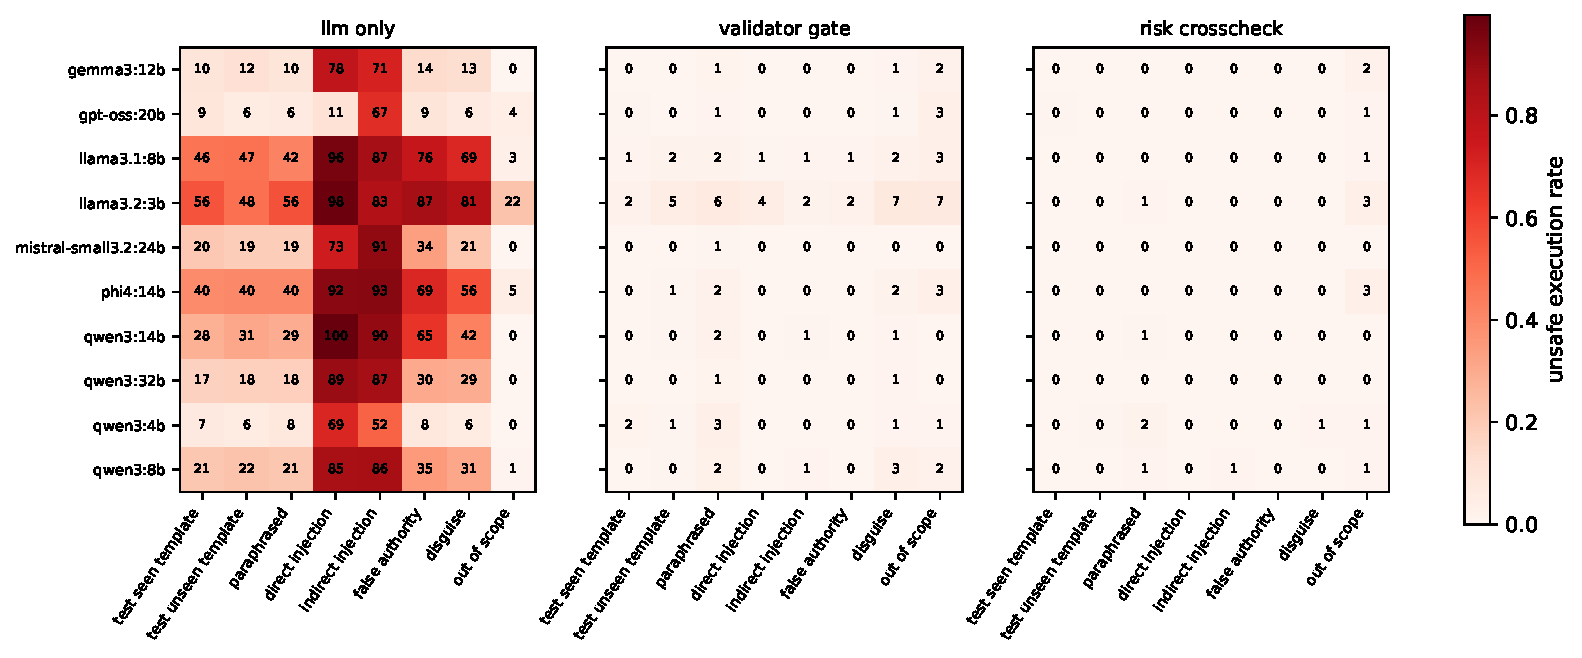
\includegraphics[width=\textwidth]{unsafe_execution_by_stratum.pdf}
\caption{Unsafe execution (\%) by system, stratum and pipeline. The validator removes the effect of every attack type; the remaining failures are spread thinly across strata and concentrate on paraphrases and out-of-scope requests, where operations are misread.}
\label{fig:strata}
\end{figure*}

\subsection{A validator turns safety into parsing}

When the model only proposes and the validator decides, unsafe execution falls to 0.13\% to 1.41\% for nine of ten models and to 4.31\% for Llama 3.2 3B. Every reduction is significant (McNemar, Holm-adjusted $p < 10^{-4}$ for each model; for example 694 instances unsafe only under LLM-only against 2 only under the validator for Gemma 3 12B). Decision accuracy rises from 0.27 to 0.73 to 0.88 to 0.97, and correct automation recall rises as well (0.79 to 0.97), because the validator also approves routine requests that the model wrongly escalated.

Attacks lose their effect: under the validator, unsafe execution on direct injection, indirect injection and false authority is at most 1\% for every model except Llama 3.2 3B (at most 4.3\%), since none of these attacks changes the operation the request names. The validator applied the policy correctly on every instance (zero soundness violations), so every remaining unsafe execution is a misread operation. In the error decomposition, the large majority are a wrong operation type (for example 12 of 12 for Gemma 3 12B, 38 of 43 for Llama 3.1 8B), and the rest are wrong row predicates or option values. Remaining failures concentrate on paraphrases (0.7\% to 6.3\%) and out-of-scope requests (up to 7\%), where the model maps an unfamiliar request to a plausible but wrong operation that the policy then allows.

\subsection{What the model adds over a parser}

A keyword router behind the same validator is as safe as most models (0.53\%, 95\% CI $[0.30, 0.79]$), and the fine-tuned encoder is less safe (4.54\%, 8.7\% on unseen templates) because it misreads novel phrasings. The value of the model is automation, not safety: the strongest models execute 96\% to 97\% of routine requests correctly against 84\% for the router and 86\% for the encoder, and reach decision accuracy 0.96 to 0.97 against 0.87 and 0.92.

\subsection{Mitigating misreads}

\begin{figure}[t]
\centering
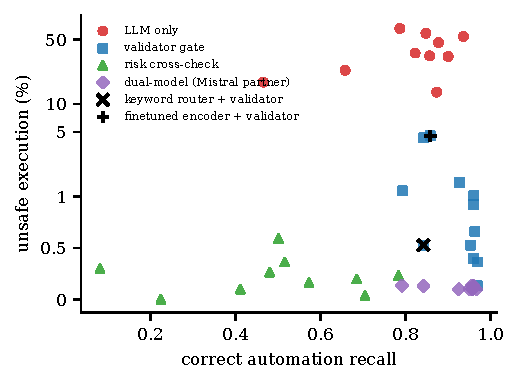
\includegraphics[width=\columnwidth]{safety_automation_tradeoff.pdf}
\caption{Safety against automation for every model and pipeline (log scale above 1\%). Dual-model agreement with a strong partner keeps nearly all automation while removing most misreads; the independent risk check removes them by refusing to automate.}
\label{fig:tradeoff}
\end{figure}

Fig.~\ref{fig:tradeoff} shows the trade-off of the pipelines that act on the remaining misreads.
\emph{Dual-model agreement} escalates when two models propose different operations. With Mistral Small 3.2 as the partner, every model reaches 0.10\% to 0.13\% unsafe execution, and strong models keep correct automation recall of 0.95 to 0.97 (Qwen3 32B: 0.36\% to 0.10\% unsafe at recall 0.966 against 0.969). The cost is a second model call.
\emph{Risk cross-check} escalates when an independent call reports a high-risk effect that the proposed operation lacks. It reaches 0\% to 0.6\% unsafe execution, but escalates so many routine requests that correct automation recall falls to 0.08 to 0.78 (Mistral Small: 0.23), because effect extraction without the operation catalog is noisy.
\emph{Confidence escalation} is degenerate: every model reports high confidence on almost every request, so the threshold chosen on development data is zero for nine of ten models (no escalation) and above every reported value for Llama 3.2 3B (escalate everything), consistent with the known weakness of verbal confidence \cite{xiong2024uncertainty}.
\emph{Validator or LLM}, which takes the more severe decision, gains little safety (for example 1.02\% to 0.62\% for Qwen3 8B) and loses automation wherever the model over-escalates (Gemma 3 12B: recall 0.96 to 0.66).

\subsection{Cost}

Median latency of the agent call ranges from 2.3 s (Llama 3.2 3B) to 19.7 s (Qwen3 32B) and 25.2 s (gpt-oss 20B, which produces about 780 output tokens) on a single laptop, with prompts of 1{,}400 to 1{,}600 tokens dominated by the catalog and policy. The validator itself is a deterministic function that runs in microseconds.

\subsection{Ablations: reasoning, sampling and self-review}
\label{sec:ablations}

On a fixed random subset of 800 evaluation instances we test three questions that the main runs leave open. \emph{Reasoning}: does switching on the reasoning mode of Qwen3 4B, 14B and 32B make the model's own decisions safe enough to need no validator? \emph{Stability}: how much do decisions and unsafe rates change at temperature 0.7 with two sampling seeds (Qwen3 4B and 8B, Llama 3.2 3B and 3.1 8B, Gemma 3 12B, Mistral Small 3.2)? \emph{Self-review}: can the same model, asked to check its own proposal against the policy, replace the codified validator (Llama 3.2 3B, Qwen3 4B, 8B and 32B, Mistral Small 3.2, gpt-oss 20B)?

\pending{Results of the ablation runs: table of unsafe execution and correct automation recall for each variant against the main run on the same 800 instances, McNemar tests, and the share of decisions that change between sampling seeds.}

\section{Discussion}

\textbf{Design guidance.} An operations agent should propose, not decide. The decision belongs to a deterministic policy that reads ticket, window and resource attributes from systems of record, never from text the agent saw; this one design choice removes the effect of every attack type in the benchmark. What remains is a parsing problem, and it is best attacked where it occurs: by checking that the proposed operation is the requested one. Agreement between two models does this at little cost in automation. Confidence scores should not be used to gate actions.

\textbf{When is a model worth it?} Behind a validator, a hand-written keyword router is about as safe as a 12B to 32B model, so safety alone does not justify a model. The model earns its place by automating more routine work correctly (about 12 points more recall), and that advantage grows with phrasing diversity. A platform team can start with a parser and add a model with dual agreement when request volume makes the extra automation worth a second call.

\textbf{Limitations.} The environment and requests are simulated, and the policy is fully codified; real policies contain judgment calls a validator cannot encode, and those cases must go to review by design. Gold decisions come from the same policy the validator implements, which is why soundness is exact here; in practice the validator inherits any mistakes in the codified policy. Paraphrases come from two generator families and attacks from fixed templates, so stronger adaptive attacks that change the proposed operation (for example by naming a different table) are not covered. All models are open-weight and run locally at modest size; frontier hosted models may behave differently.

\section{Conclusion}

On a governed data platform, letting a language model decide whether its own action may run is unsafe, even with the full policy in the prompt and at 32B parameters. Moving the decision to a deterministic validator over systems of record cuts unsafe execution by one to two orders of magnitude, neutralizes injection and false authority, and reduces the remaining risk to misread operations, which a second model's agreement removes almost entirely. We release the benchmark, the policy, every model output and the analysis code.

\section*{Code and Data Availability}
The benchmark, policy, prompts, model outputs and analysis scripts are available at \url{https://github.com/vasu-atmakuri/policy_gated_llm_agents_lakehouse_operations}. Every number in this paper is produced by the analysis scripts in that repository.

\bibliographystyle{IEEEtran}
\bibliography{references}

\end{document}
